% !TeX program = pdflatex
\documentclass[11pt,a4paper]{article}

\usepackage[
  a4paper,
  top=2.0cm,
  bottom=2.0cm,
  left=2.2cm,
  right=2.2cm
]{geometry}
\usepackage{amsmath}
\usepackage{amssymb}
\usepackage{booktabs}
\usepackage{tabularx}
\usepackage{array}
\usepackage{enumitem}
\usepackage{xcolor}
\usepackage{graphicx}
\usepackage{float}
\usepackage{caption}
\usepackage{tikz}
\usepackage{listings}
\usepackage[hidelinks]{hyperref}

\usetikzlibrary{arrows.meta, positioning, shapes.geometric}

\definecolor{titleblue}{RGB}{25,65,115}
\definecolor{lightblue}{RGB}{232,241,250}
\definecolor{lightgray}{RGB}{245,245,245}

\setlength{\parindent}{0pt}
\setlength{\parskip}{0.45em}
\renewcommand{\arraystretch}{1.22}
\setlist[itemize]{leftmargin=2em,itemsep=0.25em,topsep=0.25em}
\setlist[enumerate]{leftmargin=2.2em,itemsep=0.25em,topsep=0.25em}

\lstset{
  basicstyle=\ttfamily\small,
  backgroundcolor=\color{lightgray},
  frame=single,
  breaklines=true,
  columns=fullflexible,
  keepspaces=true,
  showstringspaces=false
}

\newcommand{\reportimage}[2]{%
  \IfFileExists{#2}{%
    \includegraphics[width=#1]{#2}%
  }{%
    \fbox{%
      \begin{minipage}[c][5.2cm][c]{#1}
        \centering
        Missing image file: \nolinkurl{#2}
      \end{minipage}%
    }%
  }%
}

\title{
  \bfseries\color{titleblue}
  LungLogic Dual-Branch Lung Model Control Software\\Stage Report
}
\author{Yuqiao Li and the LungLogic Project Team}
\date{\today}

\begin{document}
\maketitle

\begin{abstract}
This report documents the current control-layer implementation of the LungLogic prototype. It focuses on how user-facing requirements, including respiratory rate, tidal volume, inspiration-to-expiration ratio, target flow rate, and left/right asymmetry, are converted into software states, target flows, valve commands, and real-time monitoring data. Mechanical analysis is treated only as background for model parameter selection. The present software uses a first-order grey-box model as the basis for the digital twin and feedforward control. If future bench data shows significant overshoot, oscillation, delay, or inertial behaviour, the model can be upgraded to a second-order or delayed model.
\end{abstract}

\tableofcontents
\newpage

\section{Stage Objectives and Control Boundary}

The objective of this stage is to establish a runnable, tunable, and loggable dual-branch lung control software framework. The software is intended to support both simulation-stage design and later hardware closed-loop testing.

The current system boundary is:

\begin{itemize}
  \item No positive pressure source is used. During inspiration, the lung phantom expands passively by material rebound while connected to atmosphere. During expiration, a regulated vacuum source actively contracts the lung phantom.
  \item The left and right lung branches are controlled independently. Each side contains an atmosphere routing valve, a vacuum routing valve, a PPV40V proportional pinch valve, and an SFM3300 bidirectional flow sensor.
  \item The control layer uses a 100 Hz control cycle for the breathing state machine, flow PID control, volume estimation, valve interlocking, fault handling, and telemetry.
  \item The Python host software is responsible for configuration, simulation tuning, visualisation, serial communication, data logging, and post-experiment plotting.
\end{itemize}

At this stage, the output should be understood as a control and software prototype, not a final hardware validation result. Stability, leakage, pressure range, and long-term repeatability still require bench testing.

\section{Mapping User Requirements to Control Parameters}

The project requirements include adjustable respiratory rate, tidal volume, I:E ratio, inspiration/expiration flow rates, and controllable left/right imbalance. The software maps these requirements to the variables shown in Table~\ref{tab:param-map}.

\begin{table}[H]
\centering
\caption{Mapping from user settings to control variables}
\label{tab:param-map}
\begin{tabularx}{\textwidth}{
  >{\raggedright\arraybackslash}p{3.4cm}
  >{\raggedright\arraybackslash}p{4.5cm}
  X
}
\toprule
\textbf{User setting} & \textbf{Software variable} & \textbf{Control meaning} \\
\midrule
Respiratory rate & \texttt{respiratory\_rate\_bpm} & Defines the breathing period $T_c=60/RR$. The nominal value is 15 bpm, corresponding to 4 s/cycle. \\
I:E ratio & \texttt{ie\_inspiration}, \texttt{ie\_expiration} & Splits the cycle into inspiration and expiration times: $T_{in}=T_c I/(I+E)$ and $T_{out}=T_c E/(I+E)$. The nominal ratio is 1:2. \\
Tidal volume & \texttt{left\_target\_ml}, \texttt{right\_target\_ml} & Independent target volume for each lung branch. The nominal setting is 250 mL per side, or 500 mL total. \\
Target fill time & \texttt{target\_fill\_time\_s} & Converts the volume target into a target inspiration flow rate. The nominal value is 1.3 s. \\
Ventilation imbalance & Left/right targets and model parameters & Allows simulated left/right imbalance through different volume targets, time constants, or flow signs. \\
Direction-change dead time & \texttt{dead\_time\_s} & Closes all routing valves during direction changes to avoid connecting atmosphere and vacuum at the same time. \\
Precondition time & \texttt{precondition\_s} & Applies vacuum before the first cycle to establish a repeatable collapsed initial condition. \\
\bottomrule
\end{tabularx}
\end{table}

Table~\ref{tab:notation} summarises the main mathematical symbols used in the report.

\begin{table}[H]
\centering
\caption{Notation used in the control report}
\label{tab:notation}
\scriptsize
\setlength{\tabcolsep}{4pt}
\renewcommand{\arraystretch}{1.12}
\begin{tabularx}{0.96\textwidth}{
  >{\centering\arraybackslash}p{2.0cm}
  >{\raggedright\arraybackslash}p{3.2cm}
  X
}
\toprule
\textbf{Symbol} & \textbf{Meaning} & \textbf{Description} \\
\midrule
$RR$ & Respiratory rate & Breaths per minute, used to compute the breathing cycle period. \\
$T_c$ & Cycle period & $T_c=60/RR$, in seconds. \\
$I,E$ & I:E ratio terms & Inspiration and expiration ratio terms used to split the cycle. \\
$T_{in}$ & Inspiration time & $T_{in}=T_c I/(I+E)$. \\
$T_{out}$ & Expiration time & $T_{out}=T_c E/(I+E)$. \\
$T_{\mathrm{fill}}$ & Target fill time & Time used to convert tidal volume target into reference inspiratory flow. \\
$T_{dead}$ & Dead time & All-routing-valves-closed interval during direction changes. \\
$i$ & Branch index & Refers to the left or right lung branch. \\
$V_i$ & Estimated branch volume & Integrated branch volume, in mL. \\
$V^*_{T,i}$ & Target tidal volume & Branch-specific inspiration termination target, in mL. \\
$V_{\max,i}$ & Maximum model volume & Capacity limit used by the first-order branch model. \\
$V_{\mathrm{end}}$ & End-expiration volume & Volume threshold for stopping vacuum contraction. \\
$Q_i$ & Measured branch flow & SFM3300 flow in SLM; positive in inspiration and negative in expiration. \\
$Q^*_i$ & Reference flow & Target flow magnitude tracked by the PID controller. \\
$Q^*_{in,i}$ & Reference inspiratory flow & Computed from $Q^*_{in,i}=0.06V^*_{T,i}/T_{\mathrm{fill}}$. \\
$Q^*_{out,i}$ & Reference expiratory flow & Target flow magnitude during vacuum contraction. \\
$Q_{\max,i}$ & Full-open available flow & Estimated from current volume, capacity, and time constant for feedforward. \\
$\dot V_i$ & Volume rate & Related to flow by $Q_i=0.06\dot V_i$. \\
$\Delta t$ & Control time step & At 100 Hz, $\Delta t=0.01$ s. \\
$a_i$ & Normalised PPV40V opening & $a_i=0$ closed, $a_i=1$ fully open. \\
$a_{ff,i}$ & Feedforward opening & Base PPV40V opening estimated from the first-order model. \\
$U_i$ & PPV40V command voltage & $U_i=5(1-a_i)$; 0 V fully open and 5 V fully closed. \\
$\gamma$ & Valve exponent & Nonlinear exponent between PPV40V opening and effective flow. \\
$\tau_{in,i}$ & Inspiration time constant & Expansion speed when branch $i$ is connected to atmosphere. \\
$\tau_{out,i}$ & Expiration time constant & Contraction speed when branch $i$ is connected to vacuum. \\
$e_i$ & Flow error & $e_i=Q^*_i-|Q_i|$ for PID control. \\
$d_i$ & Derivative input & $d_i=-d|Q_i|/dt$, used as a damping term. \\
$K_p,K_i,K_d$ & PID gains & Proportional, integral, and derivative gains. \\
$L$ & Explicit delay & Total delay term in a possible delayed model. \\
$\omega_n,\zeta$ & Second-order parameters & Natural frequency and damping ratio for a possible second-order model. \\
\bottomrule
\end{tabularx}
\end{table}

\section{Control Logic and Mathematical Formulation}

This section reorganises the control logic as a step-by-step path from user settings to valve commands. The sequence is: breathing timing, reference flow generation, first-order lung modelling, model-based feedforward, PID feedback correction, actuator voltage conversion, and finally volume-based branch termination.

\subsection{From User Settings to Breathing Timing}

The respiratory rate defines the duration of one complete breathing cycle:

\begin{equation}
  T_c=\frac{60}{RR}.
\end{equation}

The I:E ratio then divides this cycle into inspiration and expiration:

\begin{equation}
  T_{in}=T_c\frac{I}{I+E},
  \qquad
  T_{out}=T_c\frac{E}{I+E}.
\end{equation}

For the nominal setting of 15 bpm and I:E = 1:2, the cycle time is 4 s, giving approximately 1.33 s for inspiration and 2.67 s for expiration.

\subsection{Reference Flow Generation}

The target inspiratory flow is computed from the desired tidal volume and target fill time:

\begin{equation}
  Q^*_{in,i}
  =
  0.06
  \frac{V^*_{T,i}}{T_{\mathrm{fill}}}.
\end{equation}

The factor 0.06 converts mL/s to SLM. With the nominal setting of 250 mL per side and 1.3 s fill time:

\begin{equation}
  Q^*_{in}
  =
  0.06 \times \frac{250}{1.3}
  \approx
  11.54~\mathrm{SLM}.
\end{equation}

During expiration, the measured flow is negative because the vacuum source contracts the lung phantom. The controller therefore tracks the magnitude of the flow rather than its signed value. In both inspiration and expiration, the feedback error is written as:

\begin{equation}
  e_i=Q^*_i-|Q_i|.
\end{equation}

\subsection{First-Order Lung Branch Model}

Each lung branch is modelled as a first-order variable-volume system:

\begin{equation}
\dot V_i =
\begin{cases}
a_i^\gamma (V_{\max,i}-V_i)/\tau_{in,i}, & \text{inspiration},\\
-a_i^\gamma V_i/\tau_{out,i}, & \text{expiration},\\
0, & \text{isolated}.
\end{cases}
\end{equation}

The flow-volume relationship is:

\begin{equation}
  Q_i = 0.06\dot V_i,
  \qquad
  V_i[k]=V_i[k-1]+\frac{1000}{60}Q_i[k]\Delta t.
\end{equation}

Here $V_i$ is the estimated branch volume, $V_{\max,i}$ is the maximum model volume, $\tau_{in,i}$ describes passive rebound when the branch is connected to atmosphere, and $\tau_{out,i}$ describes contraction under vacuum. The opening $a_i$ is the normalised PPV40V opening, and $\gamma$ captures the nonlinear relation between valve opening and effective flow.

\subsection{Model-Based Feedforward}

The first-order model is used to estimate a base valve opening before feedback correction is applied. This reduces the amount of work left to the PID controller:

\begin{equation}
  a_{ff,i} =
  \left(
    \frac{Q^*_i}{Q_{\max,i}}
  \right)^{1/\gamma}.
\end{equation}

During inspiration, the full-open available flow is estimated as:

\begin{equation}
  Q_{\max,i}=0.06\frac{V_{\max,i}-V_i}{\tau_{in,i}}.
\end{equation}

During expiration, it is estimated as:

\begin{equation}
  Q_{\max,i}=0.06\frac{V_i}{\tau_{out,i}}.
\end{equation}

\subsection{PID Feedback Correction}

The PID controller corrects the model-based opening using measured flow feedback:

\begin{equation}
  a_i =
  \mathrm{sat}_{[0,1]}
  \left[
    a_{ff,i}
    +K_p e_i
    +K_i\int e_i dt
    +K_d d_i
  \right].
\end{equation}

The derivative term uses the measurement derivative:

\begin{equation}
  d_i=-\frac{d|Q_i|}{dt}.
\end{equation}

This avoids differentiating the reference step directly and reduces derivative kick during state transitions. The default value is $K_d=0$, so the controller behaves like the previous PI implementation until derivative damping is tuned on hardware.

The current default controller parameters are:

\begin{itemize}
  \item $K_p=0.022~\mathrm{opening/SLM}$;
  \item $K_i=0.16~\mathrm{opening/(SLM\cdot s)}$;
  \item $K_d=0.0~\mathrm{opening\cdot s/SLM}$;
  \item integral limit: 2.0;
  \item conditional integration for anti-windup.
\end{itemize}

\subsection{Valve Command Conversion}

The PID output is an opening command, but the PPV40V receives a voltage command. The conversion used by both the simulation and hardware firmware is:

\begin{equation}
  U_i=5(1-a_i).
\end{equation}

With the current project convention, $a_i=1$ corresponds to 0 V and a fully open PPV40V, while $a_i=0$ corresponds to 5 V and a fully closed PPV40V. On the hardware, STM32 3.3 V PWM outputs pass through external low-pass and level-conversion circuits to generate the 0--5 V command.

\subsection{Volume-Based Termination and Independent Branch Control}

Flow control regulates how quickly each branch changes volume, but branch termination is based on estimated volume. During inspiration, a branch is closed when:

\begin{equation}
  V_i \geq V^*_{T,i}.
\end{equation}

Both routing solenoids on that branch close at the threshold. The PPV40V keeps
its last commanded opening for the next phase; stop or fault closes it.
During expiration, vacuum contraction stops when:

\begin{equation}
  V_i \leq V_{\mathrm{end}}.
\end{equation}

The left and right branches are evaluated independently. If one side reaches its target first, that side can close while the other continues. This is the basis for asymmetric ventilation simulation, where imbalance can be introduced through different left/right tidal-volume targets, time constants, PPV40V mappings, sensor signs, or zero offsets.

\subsection{Model Parameters and Calibration Status}

The initial model parameters were selected from the mechanical team's lung phantom and tubing report. The report approximated rebound as:

\begin{equation}
  V(t)=V_{\max}(1-e^{-t/\tau}).
\end{equation}

The reported geometry gave a maximum displaced volume of approximately 558 mL. For 10 mm inner diameter tubing, the reported recovery time was approximately $4\tau=2.27$ s, giving:

\begin{equation}
  \tau_{in}\approx 2.27/4 \approx 0.57~\mathrm{s}.
\end{equation}

The current initial parameter set is:

\begin{itemize}
  \item left and right $V_{\max}=558$ mL;
  \item left $\tau_{in}=0.57$ s and right $\tau_{in}=0.60$ s;
  \item left/right $\tau_{out}=0.50/0.54$ s;
  \item valve exponent $\gamma=1.15$;
  \item transport delay = 25 ms;
  \item sensor time constant = 20 ms;
  \item flow noise = 0.10 SLM.
\end{itemize}

These values are initial simulation assumptions rather than final hardware calibration results. At the hardware stage, PPV40V voltage-flow tests should be used to update $\gamma$ or replace it with a lookup table, valve-step tests should estimate transport delay, SFM3300 step responses should identify sensor dynamics, and steady zero-flow/steady-flow recordings should estimate sensor noise.

\subsection{Conditions for Upgrading to a Second-Order Model}

The first-order model is suitable for early control design because it is simple and easy to identify from bench data. A second-order or delayed model should be considered if hardware tests show clear underdamped flow oscillation, a rising edge that cannot be fitted by a first-order response, significant PPV40V mechanical lag, or strong coupling between the two branches.

A possible second-order form is:

\begin{equation}
  G(s)=\frac{\omega_n^2}{s^2+2\zeta\omega_n s+\omega_n^2}e^{-Ls},
\end{equation}

where $\omega_n$ is the natural frequency, $\zeta$ is the damping ratio, and $L$ is an explicit delay.

\section{Control State Machine}

The breathing cycle is divided into multiple states rather than only inspiration and expiration. This ensures valve interlocking, avoids direct atmosphere-vacuum cross-flow, and establishes a repeatable initial condition.

\begin{figure}[H]
\centering
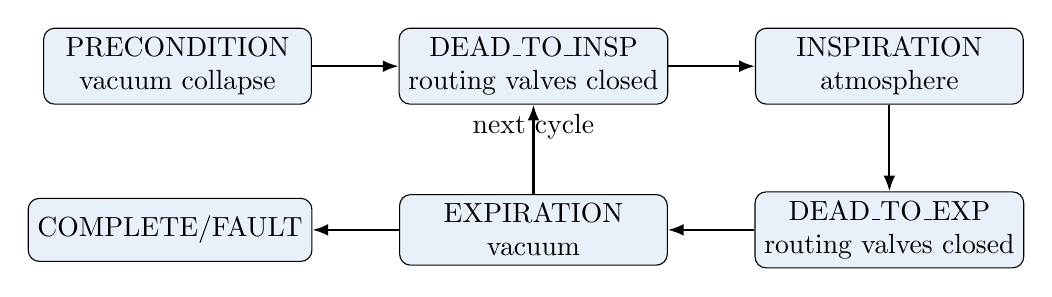
\begin{tikzpicture}[
  node distance=11mm,
  state/.style={draw, rounded corners, align=center, minimum width=34mm, minimum height=8mm, fill=lightblue},
  arrow/.style={-{Latex[length=2mm]}, thick}
]
\node[state] (pre) {PRECONDITION\\vacuum collapse};
\node[state, right=of pre] (dti) {DEAD\_TO\_INSP\\routing valves closed};
\node[state, right=of dti] (insp) {INSPIRATION\\atmosphere};
\node[state, below=of insp] (dte) {DEAD\_TO\_EXP\\routing valves closed};
\node[state, left=of dte] (exp) {EXPIRATION\\vacuum};
\node[state, left=of exp] (done) {COMPLETE/FAULT};

\draw[arrow] (pre) -- (dti);
\draw[arrow] (dti) -- (insp);
\draw[arrow] (insp) -- (dte);
\draw[arrow] (dte) -- (exp);
\draw[arrow] (exp) -- node[above]{next cycle} (dti);
\draw[arrow] (exp) -- (done);
\end{tikzpicture}
\caption{Breathing state machine used by the current control software}
\end{figure}

\begin{table}[H]
\centering
\caption{Valve behaviour in each state}
\begin{tabularx}{\textwidth}{p{3.2cm}p{2.8cm}p{2.8cm}X}
\toprule
\textbf{State} & \textbf{Atmosphere valve} & \textbf{Vacuum valve} & \textbf{Control objective} \\
\midrule
PRECONDITION & closed & open & Collapse the lung phantom to a repeatable initial condition. \\
DEAD\_TO\_INSP & closed & closed & Direction-change dead time. \\
INSPIRATION & open & closed & Regulate positive flow until the target tidal volume is reached. \\
DEAD\_TO\_EXP & closed & closed & Direction-change dead time before vacuum contraction. \\
EXPIRATION & closed & open & Regulate negative flow until end-expiration volume is reached. \\
COMPLETE/FAULT & closed & closed & Stop the run or enter a safe state. \\
\bottomrule
\end{tabularx}
\end{table}

At no point should the atmosphere and vacuum valves on the same branch be open simultaneously. This is checked in both the simulation logic and the STM32 firmware.

\section{Control Software Implementation}

\subsection{Simulation Implementation: \texttt{lung\_pid\_gui.py}}

\texttt{lung\_pid\_gui.py} is the simulation-stage GUI. It does not directly control STM32 or physical valves. Instead, it calls the first-order model and state machine in \texttt{lung\_model.py} to generate a repeatable digital-twin result. Its purpose is to verify the control intent, parameter ranges, and state transitions before hardware testing.

The simulation GUI currently provides:

\begin{itemize}
  \item adjustment of respiratory rate, I:E ratio, left/right tidal volume targets, target fill time, and simulation cycles;
  \item adjustment of PID gains, integral limit, and model feedforward;
  \item adjustment of branch capacity, inspiration and expiration time constants, valve exponent, transport delay, sensor noise, and dead time;
  \item a dynamic pneumatic diagram showing atmosphere, vacuum, routing valves, PPV40V, SFM3300, and both lung branches;
  \item time histories of volume, flow, PPV opening, and state;
  \item a live monitor window showing flow rate, reference flow, volume, PPV opening, command voltage, routing valves, and live flow curves.
\end{itemize}

The word ``live'' in the simulation GUI means live playback of precomputed simulation data. It is not hardware telemetry from SFM3300 sensors.

\begin{figure}[H]
\centering
\reportimage{0.7\textwidth}{sim1.png}
\caption{Current simulation GUI showing the parameter panel, Dynamic Model view, and Live Curves tab}
\label{fig:simulation-gui}
\end{figure}

\begin{figure}[H]
\centering
\reportimage{0.7\textwidth}{sim2.png}
\caption{Simulation-stage live monitor showing state, cycle number, measured and reference flow, volume, PPV command, routing valves, and rolling flow curve}
\label{fig:live-monitor}
\end{figure}

In addition, \texttt{lung\_pid\_simulation.py} provides a command-line simulation path that writes \texttt{output/lung\_simulation.csv} and \texttt{output/lung\_simulation.png}. This allows the same model to support both GUI demonstration and batch simulation.

\subsection{Hardware Monitor and Serial Protocol: \texttt{lung\_hardware\_monitor.py} and STM32 Firmware}

\texttt{lung\_hardware\_monitor.py} is the hardware-facing host program. It sends the same configuration parameters to the NUCLEO-G474RE, starts the physical control loop, receives SFM3300/controller telemetry, saves CSV logs, and produces result plots. It is the main software path from simulation to hardware testing.

The serial workflow is:

\begin{enumerate}
  \item The host opens the serial port and sends \texttt{HELLO}.
  \item STM32 replies with \texttt{READY,LUNGLOGIC\_G474,2}.
  \item The host sends \texttt{CFG,2}, including breathing parameters, PID gains, volume limits, model parameters, and valve exponent.
  \item After acknowledgement, the host sends \texttt{START}.
  \item During operation, the host sends \texttt{PING} as a keep-alive signal, while STM32 sends \texttt{TEL} telemetry at 50 Hz.
  \item The host saves CSV data and plots volume, flow, and PPV opening.
\end{enumerate}

Telemetry includes state, cycle index, measured left/right flow, estimated left/right volume, reference flow, PPV opening, command voltage, and valve mask.

The STM32 firmware \texttt{firmware/lung\_controller\_stm32/lung\_controller\_stm32.ino} currently implements:

\begin{itemize}
  \item 100 Hz control loop;
  \item TCA9548A/PCA9548A Pa.Hub channel selection for the two SFM3300 sensors;
  \item D10/D9 3.3 V PWM outputs converted by external low-pass and level-shifting circuits into two 0--5 V PPV40V commands;
  \item D6 active-low emergency stop input;
  \item four interlocked solenoid valve outputs;
  \item the same state machine and PID structure as the Python model;
  \item fault checks for sensor read failure, flow limit, volume limit, host timeout, and valve interlock;
  \item safe fault action: close all routing valves and command the PPV40V valves to approximately 5 V.
\end{itemize}

The closed-loop firmware uses the PCB profile 0 NUCLEO-G474RE allocation:

\begin{table}[H]
\centering
\caption{NUCLEO-G474RE pin mapping used by the current hardware firmware}
\begin{tabular}{lll}
\toprule
\textbf{Pin} & \textbf{Function} & \textbf{Type} \\
\midrule
D2 & Right VAC solenoid valve & digital output \\
D3 & Left VAC solenoid valve & digital output \\
D4 & Right ATM solenoid valve & digital output \\
D5 & Left ATM solenoid valve & digital output \\
D6 & Emergency stop input & digital input, active-low \\
D9 & Right PPV40V command & 3.3 V PWM through external 0--5 V interface \\
D10 & Left PPV40V command & 3.3 V PWM through external 0--5 V interface \\
A4/PC1 & Software-I2C SDA & open-drain communication \\
A5/PC0 & Software-I2C SCL & open-drain communication \\
\bottomrule
\end{tabular}
\end{table}

The 24 V solenoid valves and PPV40V power cannot be driven directly from STM32 pins. They require suitable MOSFET stages, flyback protection, external power, and a shared ground. The G474RE's 3.3 V PWM also requires a validated 0--5 V conversion stage. Software safety checks do not replace a mechanical vacuum regulator or a hardware emergency stop.

\section{Hardware Migration and Calibration Plan}

When moving from simulation to hardware, the control logic can remain mostly the same, but the model parameters, sensor offsets, valve mapping, and safety limits must be calibrated experimentally. The current codebase provides three main entry points:

\begin{itemize}
  \item \texttt{config.example.json}: shared configuration for simulation and hardware;
  \item \texttt{lung\_hardware\_monitor.py}: sends configuration to STM32 and records telemetry;
  \item \texttt{fit\_lung\_parameters.py}: fits first-order time constants from CSV data.
\end{itemize}

\subsection{From Simulation Parameters to Hardware Commands}

In hardware mode, the user settings are translated in the same way:

\begin{itemize}
  \item respiratory rate and I:E ratio become inspiration, expiration, and cycle times;
  \item left/right tidal volume targets become branch-specific volume termination conditions;
  \item target fill time becomes target inspiration flow;
  \item dead time becomes the all-valves-closed interval between inspiration and expiration;
  \item PID and model parameters become PPV40V PWM duty cycles, which are filtered into 0--5 V command voltages.
\end{itemize}

The inspiration/expiration switching gap is manually adjustable through \texttt{dead\_time\_s}. In the GUI it appears as \texttt{Direction-change dead time / s}; in STM32 it is sent as \texttt{deadTimeMs}.

\subsection{Required Calibrations}

\paragraph{1. SFM3300 zero-flow offset calibration.}
When all routing valves are closed, the true flow should be 0 SLM. Real sensors may still report a small offset. If this offset is integrated, the estimated volume will drift. A recommended calibration is to average the measured flow during each dead-time interval and subtract it:

\begin{equation}
  Q_{\mathrm{corrected},i}=Q_{\mathrm{measured},i}-Q_{\mathrm{offset},i}.
\end{equation}

\paragraph{2. Atmospheric rebound time constant \texorpdfstring{$\tau_{in}$}{tau\_in}.}
This parameter describes how fast the fake lung re-expands after being compressed or vacuum-collapsed and then connected to atmosphere. The current value of approximately 0.57 s comes from the mechanical team's 10 mm tubing test. The test should be repeated with the final hardware by fully opening the PPV40V, opening the atmosphere valve, recording SFM3300 flow, integrating volume, and fitting the first-order model. The 1.3 s target fill time is normally kept fixed unless the lung material rebound degrades significantly.

\paragraph{3. Vacuum contraction time constant \texorpdfstring{$\tau_{out}$}{tau\_out}.}
This parameter describes how fast the vacuum source contracts the lung phantom. It is currently an initial placeholder and must be updated using controlled vacuum tests.

\paragraph{4. PPV40V voltage-flow calibration.}
The PPV40V command voltage and actual flow are not perfectly linear. The current model approximates:

\begin{equation}
  Q \propto a^\gamma,
  \qquad
  U=5(1-a).
\end{equation}

Hardware step tests should scan 0--5 V commands in both inspiration and expiration directions. If the exponent model is sufficient, update \texttt{valve\_exponent}. If there is strong nonlinearity or a dead zone, a lookup table or piecewise map should be used.

\paragraph{5. Sensor delay, noise, and direction calibration.}
The signs, noise levels, and response delays of the two SFM3300 sensors must be verified. The current delay and noise values are initial assumptions.

\paragraph{6. Left/right branch consistency calibration.}
The two branches should be calibrated independently. The final system should have separate left/right \texttt{tau\_in}, \texttt{tau\_out}, flow sign, zero offset, and PPV mapping values.

\subsection{Role of \texttt{lung\_hardware\_monitor.py}}

\texttt{lung\_hardware\_monitor.py} has three roles in hardware migration.

First, it is a configuration tool. It reads \texttt{config.example.json} and sends the full \texttt{CFG} command to STM32.

Second, it is a run-control tool. It sends \texttt{START}, \texttt{STOP}, and periodic \texttt{PING} messages.

Third, it is the source of calibration data. It records \texttt{TEL} telemetry to CSV, including measured flow, estimated volume, reference flow, opening, command voltage, state, and valve mask. These CSV files can be used by \texttt{fit\_lung\_parameters.py} and later cycle-analysis tools.

\subsection{Future Calibration Interface}

The current hardware calibration workflow is script- and CSV-based. Future GUI support may include:

\begin{itemize}
  \item manual dead-time setting and testing;
  \item PPV40V fully-open recovery tests and automatic time-to-250-mL calculation;
  \item vacuum contraction tests and automatic \texttt{tau\_out} fitting;
  \item PPV40V 0--5 V step scanning;
  \item per-cycle zero-flow offset estimation;
  \item automatic tidal volume error, cycle timing error, left/right balance error, and $\pm3\%$ stability reporting.
\end{itemize}

\section{Compliance with Scope}

Table~\ref{tab:scope} summarises the current control-layer status relative to the project scope.

\begin{table}[H]
\centering
\caption{Current control-layer compliance with scope}
\label{tab:scope}
\begin{tabularx}{\textwidth}{
  >{\raggedright\arraybackslash}p{4.7cm}
  >{\centering\arraybackslash}p{2.5cm}
  X
}
\toprule
\textbf{Requirement} & \textbf{Status} & \textbf{Comment} \\
\midrule
12--18 bpm, nominal 15 bpm & Implemented & Supported by GUI and configuration file. \\
500 mL nominal tidal volume & Implemented in simulation & Default is 250 mL per side; hardware validation is still required. \\
Adjustable I:E ratio, nominal 1:2 & Implemented & RR and I:E determine inspiration and expiration times. \\
Independent left/right control & Implemented in control logic & Separate targets, PID control, termination, and valve commands. \\
Controllable ventilation imbalance & Implemented in software & Achieved through left/right target and model parameter differences. \\
Real-time adjustment and visualisation & Implemented on host side & GUI supports parameter setting, dynamic model, curves, and live monitor. \\
Data acquisition and analysis & Partially implemented & CSV logging and plotting exist; automatic abnormality metrics still need work. \\
Cycle-to-cycle recalibration & Partially implemented & Preconditioning and controller reset exist; automatic zero-flow offset estimation is not complete. \\
$\pm3\%$ stability & To be verified & Requires repeated hardware cycle statistics. \\
Pressure range and leakage proof & To be verified & Current software has no pressure sensor input or leakage test result. \\
\bottomrule
\end{tabularx}
\end{table}

\section{Current Limitations and Next Steps}

The current software expresses the intended control behaviour, but several limitations remain:

\begin{itemize}
  \item $\tau_{out}$, PPV40V nonlinearity, and sensor dynamics are still initial values;
  \item automatic per-cycle zero-flow offset estimation has not yet been added;
  \item the simulation GUI is not equivalent to hardware telemetry;
  \item an automatic compliance report is not yet implemented;
  \item without pressure sensor input, software alone cannot prove pressure safety.
\end{itemize}

Recommended next steps are:

\begin{enumerate}
  \item use SFM3300 data to re-identify $\tau_{in}$ and $\tau_{out}$;
  \item perform PPV40V 0--5 V step tests to fit voltage-flow mapping;
  \item add dead-time zero-flow offset estimation to STM32 firmware;
  \item add Python cycle analysis for RR, I:E, tidal volume error, left/right balance, and stability;
  \item connect the GUI live monitor to real hardware telemetry;
  \item upgrade to a second-order or delayed model if first-order behaviour is insufficient.
\end{enumerate}

\section{Conclusion}

The current LungLogic control layer provides a complete software path from user requirements to control actions. Respiratory rate, tidal volume, and I:E ratio are converted into cycle timing and reference flows. A state machine safely switches between preconditioning, dead time, inspiration, and expiration. A feedforward plus PID controller converts the target flow into PPV40V opening, and volume-based termination supports symmetric or asymmetric ventilation.

The host-side GUI supports parameter adjustment, digital-twin visualisation, real-time simulated flow monitoring, and curve display. The hardware monitor and STM32 firmware provide serial configuration, telemetry logging, PWM-based PPV40V command output, emergency stop input, and basic fault protection.

The main value of this stage is the implementation of the control logic and software workflow. Final performance claims still require hardware data from the SFM3300 sensors, updated model parameters, and cycle-level analysis tied directly to the project scope.

\begin{thebibliography}{9}

\bibitem{orifice}
Mechanical design team, \textit{System Dynamics and Volume Constraints / Orifice Report}, 2026.

\bibitem{electrical}
Electrical design team, \textit{LungLogic Week 4 Progress Report: Electrical Section}, 2026.

\bibitem{software}
LungLogic codebase: \texttt{lung\_model.py}, \texttt{lung\_pid\_gui.py}, \texttt{lung\_hardware\_monitor.py}, and \texttt{firmware/lung\_controller\_stm32/lung\_controller\_stm32.ino}, 2026.

\bibitem{scope}
LungLogic project scope document, 2026.

\end{thebibliography}

\end{document}
